% !TEX root = ../dg.tex

\section{Tangent Vectors}

Notice that there's nothing in \cref{def:manifold} that says that a manifold has to live inside some bigger Euclidean space. This is in contrast to a typical undergraduate differential geometry course (like MATH 474 here at CSU), which is typically focused on surfaces in $\R^3$. 

Of course, many manifolds (like spheres) do naturally live in some Euclidean space, and it turns out that the Whitney embedding theorem~\cite{whitneySelfintersectionsSmooth$n$manifold1944,whitneySingularitiesSmooth$n$manifold1944} guarantees that all manifolds \emph{can} be embedded in some Euclidean space, but this embedding is not necessarily going to be pleasant to work with. If you've encountered them before, it is often much easier to work with projective spaces and Grassmannians \emph{without} embedding them anywhere in particular.

Since our manifolds don't necessarily live inside a Euclidean space, we have to be a bit careful about what a tangent vector at a point is supposed to be. In particular, a tangent vector at a point lives in a different universe than the point itself: the point is a point in the manifold, but the tangent vector does \emph{not} live on the manifold. This is clear even on a sphere in Euclidean space: the tangent vector to a point on the sphere does not live on the sphere! However, in Euclidean space we can kind of cheat and think of both the point and the tangent vector as both living inside the ambient Euclidean space. In general, we can't get away with this.

Now even in Euclidean space you have to be a little careful with this mixing of point and tangent vector: the tangent vector can't be any \emph{arbitrary} vector in the ambient Euclidean space: it has to lie in the \emph{tangent space} at the point, which we usually visualize as some plane which is tangent to the sphere at the point. But if we're not in Euclidean space, things are even worse: if there's supposed to be some subspace which is ``tangent at a point,'' where does it even live? Surely not in the manifold itself, but we're not thinking of the manifold as sitting inside some bigger space, so there's no ``outside'' where it can be.

This is a surprisingly nontrivial issue, requiring us to construct some abstract vector space which doesn't really live anywhere in particular. The construction is fairly non-obvious, and feels like a sneaky trick the first few times you encounter it. This is one of those situations where it seems like you're turning a concept inside-out; at least for me, the first time I encountered the following way of thinking, it made me feel uncomfortable in a similar way to when I first encountered the natural embedding of a vector space into its double dual. I will say that at some point my brain switched from ``this is weird and awkward'' to ``this is obviously the right way to do it'' and I think most differential geometers have had similar experiences, so this is something you can eventually develop intuition for.

Given that preamble, what's the idea? We're going to work by analogy with a way of thinking about vectors in $\R^n$ that's slightly different from what you may be used to. In words, we'll identify a vector $\vec{v} \in \R^n$ with the operator on differentiable functions which gives the directional derivative (in the direction of $\vec{v}$) of a function. 

That's a little vague, so let's try to characterize a tangent vector $\vec{v}$ to a point $p \in \R^n$ in this way (here I'm using the notation $p$ rather than $\vec{p}$, because I'm just thinking of $p$ as a point in a manifold, not as an element of a vector space). Given $\vec{v}$, I claim we can find some smooth curve $\alpha\from (-\epsilon, \epsilon) \to \R^n$ with $\alpha(0) = p$ and $\alpha'(0) = \vec{v}$; see \cref{fig:tangent vector curve}. In coordinates, if
\[
	\alpha(t) = (x_1(t), \dots , x_n(t)) \quad \text{for } t \in (-\epsilon, \epsilon),
\]
where the coordinate functions $x_i\from (-\epsilon,\epsilon) \to \R$ are themselves smooth, then
\[
	\alpha'(0) = (x_1'(0), \dots , x_n'(0)) = \vec{v}.
\]

\begin{figure}[htbp]
	\centering
		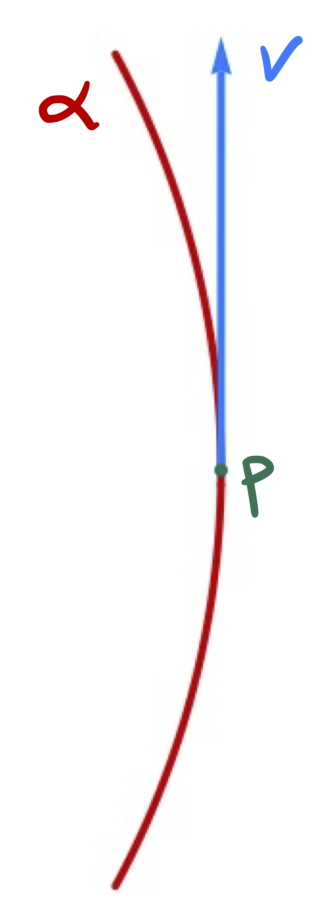
\includegraphics[height=2in]{tangent-vector-curve}
	\caption{A curve through $p$ with velocity $\vec{v}$ at $p$.}
	\label{fig:tangent vector curve}
\end{figure}

(In this specific case, we could take $\alpha(t) = p + t\vec{v}$, but it turns out not to matter which curve satisfying $\alpha(0) = p$ and $\alpha'(0) = \vec{v}$ we take.)

Now, say $f: U \to \R$ is differentiable, where $U \subseteq \R^n$ is some neighborhood of $p$. Then the directional derivative of $f$ at $p$ in the direction of $\vec{v}$ is 
\[
	\left. \frac{d(f \circ \alpha)}{dt} \right|_{t=0} = \sum_{i=1}^n \left.\frac{\partial f}{\partial x_i}\right|_p \left. \frac{d x_i}{dt} \right|_{t=0} = \left(\sum_{i=1}^n x_i'(0) \frac{\partial}{\partial x_i}]\right)f
\]
by the Chain Rule. 

On the right hand side above, we've written the directional derivative as an operator $L = \sum_{i=1}^n x_i'(0) \frac{\partial}{\partial x_i}$ acting on $f$. Moreover, this operator depends uniquely on $\vec{v}$ and is a \emph{linear derivation}, meaning that:
\begin{enumerate}
	\item $L(f + \lambda g) = L(f) + \lambda L(g)$ for all $f$ and $g$ differentiable in a neighborhood of $p$ and all $\lambda \in \R$;
	\item $L(f g) = f(p) L(g) + g(p) L(f)$ (i.e., the Product Rule).
\end{enumerate}

If it's not clear to you, it's worth looking at the above and convincing yourself that the operator $L$ didn't really depend on the choice of $\alpha$: it really only depends on $p$ and $\vec{v}$ (you may need to go back to the justification from MATH 517 that the directional derivative is well-defined).

The upshot is that, given a point $p$ and a tangent vector $\vec{v}$ at $p$, we get a directional derivative operator $L$. And, conversely, if we know how to compute a directional derivative, we (at least implicitly) know the direction, so this is really a bijective correspondence.

The benefit of thinking in this way is that we can talk about differential operators like $L$ on any manifold; after all, manifolds locally look like $\R^n$ by definition. So, with that long preamble in mind, here's the definition of a tangent vector:

\begin{definition}\label{def:tangent vector}
	Let $M^n$ be a manifold. A smooth function $\alpha\from (-\epsilon, \epsilon) \to M$ is a (smooth) curve in $M$. Suppose $\alpha(0) = p \in M$ and let $\mathcal{D}_p$ be the set of function on $M$ that are differentiable in a neighborhood of $p$. The \emph{tangent vector} to a curve $\alpha$ at $t=0$ is a function $\alpha'(0)\from \mathcal{D}_p \to \R$ given by
	\[
		\alpha'(0)f := \left. \frac{d(f\circ \alpha)}{dt} \right|_{t=0} = (f\circ \alpha)'(0).
	\] 
	A \emph{tangent vector at $p$} is the tangent vector at $t=0$ of some curve $\alpha\from (-\epsilon, \epsilon) \to M$ with $\alpha(0) = p$.
	
	The set of all tangent vectors at $p$ is the \emph{tangent space} to $M$ at $p$, denoted $T_pM$.
\end{definition}

This is a nice coordinate-free way of defining things, but it's not very useful for computations. We usually \emph{do} want to work in coordinates for computations (and certainly for any computations that we want to do on the computer), so let's see what all this means in local coordinates.

Say that $(U,\phi)$ is a coordinate chart containing $p \in M$ so that $\phi(\vec{0}) = p$, that $\alpha \from (-\epsilon , \epsilon) \to M$ is smooth with $\alpha(0) = p$, and that $f$ is a differentiable function in a neighborhood of $p$. Then
\[
	(\phi^{-1} \circ \alpha)(t) = (x_1(t), \dots , x_n(t))
\]
for some smooth functions $x_1 , \dots , x_n\from (-\epsilon, \epsilon) \to M$. Then
\[
	\alpha'(0) f = \left. \frac{d(f \circ \alpha)}{dt} right_{t = 0} = \left. \frac{d}{dt} (f \circ \phi(x_1(t),\dots , x_n(t))) \right|_{t=0} = \left.\sum_{i=1}^n x_i'(0) \frac{\partial f}{\partial x_i}\right|_{\vec{0}} = \left( \sum_{i=1}^n x_i'(0) \frac{\partial }{\partial x_i}\right|_{\vec{0}}\right)f,
\]
where I'm using a very common abuse of notation in the second expression to thinkg of $f$ as being a function on the coordinate chart $U$, and hence a function of coordinates $x_1, \dots , x_n$ (of course, it's really $f \circ \phi$ which is a function of $x_1, \dots , x_n$, as we see in the middle expression).

This all means that we can write the tangent vector $\alpha'(0) \in T_pM$ in local coordinates as
\[
	\alpha'(0) = \sum_{i=1}^n x_i'(0) \left(\frac{\partial}{\partial x_i}\right)_{\vec{0}}.
\]
Since the $x_i'(0)$ are just scalars, what we're doing here is writing $\alpha'(0)$ in terms of the \emph{local coordinate basis} $\left\{\left(\frac{\partial}{\partial x_1}\right)_{\vec{0}}, \dots , \left(\frac{\partial}{\partial x_n}\right)_{\vec{0}}\right\}$ for $T_pM$ associated to the chart $(U,\phi)$.

\begin{remark}
	In practice, we will almost always drop the subscript $\vec{0}$ and just write the basis as $\left\{\frac{\partial}{\partial x_1}, \dots , \frac{\partial}{\partial x_n}\right\}$ and generic tangent vectors as $\sum_{i=1}^n a_i \frac{\partial}{\partial x_i}$.
\end{remark}

\begin{exercise}
	Suppose a point $p \in M$ lies in two different coordinate charts. How are the two different local coordinate bases related?
\end{exercise}

It's extremely important to keep in mind that, if $p$ and $q$ are distinct points on $M$, then the tangent spaces $T_pM$ and $T_qM$ are \emph{completely different vector spaces} that in principle have nothing to do with each other (they're both vector spaces of the same dimension, and hence abstractly isomorphic, but that's essentially all we can know without more detailed information about the geometry of $M$).

Nonetheless, we often want to talk about all tangent spaces at once, so we smush them together:

\begin{definition}\label{def:tangent bundle}
	The \emph{tangent bundle} of a manifold $M$, denoted $TM$, is the (disjoint) union of tangent spaces
	\[
		TM := \bigsqcup_{p \in M} T_p M.
	\]
	Likewise, if $(T_pM)^\ast$ is the dual of $T_pM$, then the \emph{cotangent bundle} is the union of cotangent spaces
	\[
		T^\ast M := \bigsqcup_{p \in M} (T_pM)^\ast.
	\]
\end{definition}

Notice that there are natural projections $\pi: TM \to M$ and $\widetilde{\pi}: T^\ast M \to M$ which just record the base point; in other words, $\pi$ sends a tangent vector at a point to the point (formally, $TM$ and $T^\ast M$ are \emph{vector bundles}, and this projection is part of their definition).

\begin{theorem}\label{thm:tangent bundles are manifolds}
	If $M$ is an $n$-dimensional manifold, then $TM$ and $T^\ast M$ are $2n$-dimensional manifolds.
\end{theorem}

\begin{exercise}
	Prove \cref{thm:tangent bundles are manifolds}.
\end{exercise}

$T^\ast M$ is, in some sense, the most basic example of a \emph{symplectic manifold}. In physics and dynamical systems language, if $M$ is the \emph{configuration space}\footnote{Meaning it records the positions of particles; for example if we're doing dynamics of $n$ points on the circle, the configuration space is the $n$-torus $S^1 \times \dots \times S^1 = (S^1)^n$.} of a (classical) system, then $T^\ast M$ is \emph{phase space} or \emph{position-momentum space}: this is the natural setting of Hamiltonian mechanics.

\begin{example}
	$T \R^n \cong \R^n \times \R^n \cong \R^{2n}$.
\end{example}

\begin{example}
	$T S^1 \cong S^1 \times \R$, the infinite cylinder.
\end{example}

\begin{example}
	$TS^2$ is a \emph{non-trivial} bundle over $S^2$, meaning that it is \emph{not} homeomorphic to $S^2 \times \R^2$. In particular, one can show that $US^2$, which is the \emph{unit} tangent bundle (the subset of the tangent bundle consisting only of unit tangent vectors) is homeomorphic to $\SO(3) \cong \RP^3$, the real projective space, which is a circle bundle over $S^2$ different from the trivial circle bundle $S^2 \times S^1$. (For those that have taken graduate topology, $\pi_1(S^2 \times S^1) \cong \Z$, whereas $\pi_1(\RP^3) \cong \Z/2\Z$.)
\end{example}